% Universidade Aberta
% Template TeX para relatório de trabalhos
% 2024
%
%
% Dados para a capa
\newcommand{\Titulo}{Título}
\newcommand{\Ano}{2024}
\newcommand{\Autor}{Autor}
%
%
\documentclass[12pt,a4paper,final]{article}
\usepackage[stretch=10]{microtype}
\usepackage{csquotes}
\usepackage[portuguese]{babel}
\usepackage{polyglossia}
\setdefaultlanguage{portuguese}
\usepackage{graphicx}
\graphicspath{ {./images/} }
\usepackage[a4paper,top=3cm,bottom=3cm,left=3.5cm,right=2cm]{geometry}
\usepackage{booktabs}
\usepackage{newtxtext}
\usepackage{newtxmath}
\usepackage{pgf-umlsd}
\usepackage[pdfauthor=\Autor,
    pdftitle=\Titulo,
    colorlinks=true,
    linkcolor=black,
    citecolor=black,
    bookmarksopen=true]{hyperref}
\hypersetup{colorlinks, citecolor=black, urlcolor=black}
\usepackage{bookmark}
\usepackage{float}
\usepackage[style=apa, backend=biber, sortcites, url=true]{biblatex}
\addbibresource{ref.bib}
\renewcommand{\baselinestretch}{1.5}
\begin{document}
    \title{\Titulo}
    \author{\Autor}
    \date{\Ano}
    \pagenumbering{gobble}
    \begin{titlepage}
        \begin{center}
            \vspace*{4cm}

            \textbf{\large UNIVERSIDADE ABERTA}

            \textbf{\large UNIVERSIDADE DE TRÁS-OS-MONTES E ALTO DOURO}

            \vspace{1cm}

            \begin{minipage}{0.4\textwidth}
                \centering
                
\includegraphics[width=0.8\textwidth]{uab}
            \end{minipage}
            \begin{minipage}{0.4\textwidth}
                \centering
                
\includegraphics[width=0.8\textwidth]{utad}
            \end{minipage}

            \vspace{1.5cm}

            \textbf{\large \Titulo}

            \vspace{1.5cm}

            \textbf{\large \Autor}

            \vspace{2cm}

            \textbf{\large Mestrado em Engenharia Informática e Tecnologia Web}
            \vfill
            \textbf{\Ano}
        \end{center}
    \end{titlepage}
    \renewcommand{\contentsname}{Índice}
    \cleardoublepage
    \pagenumbering{roman}
    \tableofcontents
    \newpage
    \listoffigures
    \newpage
    \listoftables
    \newpage
    \cleardoublepage
    \pagenumbering{arabic}


    \section{Introdução}\label{sec:introducao}
    Este é o texto da introdução.

    \begin{figure}[H]
        \centering
        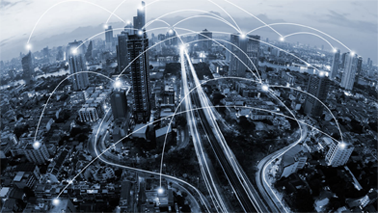
\includegraphics[width=0.9\textwidth]{img_meitw}
        \caption{Exemplo de uma figura}
        \label{fig:exemplo}
    \end{figure}


    \section{Metodologia}\label{sec:metodologia}
    Este é o texto da metodologia.

    \begin{figure}[H]
        \centering
        \begin{sequencediagram}
            \newthread{t}{:Thread}
            \newinst[1]{i}{:Instance}
            \begin{sdblock}{Block}{description}
                \begin{call}{t}{function()}{i}{}
                \end{call}
            \end{sdblock}
        \end{sequencediagram}
        \caption{Diagrama de Sequência Exemplo}
        \label{fig:diagrama-sequencia}
    \end{figure}

    \begin{enumerate}
        \item Item 1
        \item Item 2
        \item Item 3
    \end{enumerate}


    \section{Descrição}\label{sec:descricao}
    Detalhes da descrição da metodologia.

    \begin{itemize}
        \item Item 1
        \item Item 2
        \item Item 3
    \end{itemize}


    \section{Estado da Arte}\label{sec:estado-da-arte}

    \subsection{Pesquisa}\label{subsec:pesquisa}
    Detalhes da pesquisa sobre o estado da arte.

    \subsection{Critérios}\label{subsec:criterios}
    Critérios da pesquisa sobre o estado da arte.


    \section{Resultados}\label{sec:resultados}
    Este é o texto dos resultados.

    \begin{table}[H]
        \centering
        \resizebox{0.2\columnwidth}{!}{%
            \begin{tabular}{@{}|c|cccc|@{}}
                \toprule
                & A & B & C & D \\ \midrule
                X & 4 & 3 & 2 & 1 \\ \midrule
                Y & 2 & 3 & 4 & 5 \\ \midrule
                Z & 4 & 3 & 2 & 1 \\ \bottomrule
            \end{tabular}%
        }
        \caption{Tabela Exemplo}
        \label{tab:my-table}
    \end{table}


    \section{Conclusões}\label{sec:conclusoes}
    Este é o texto da conclusão com uma citação \cite{su15010857}.

    \newpage
    \printbibliography
\end{document}
